\documentclass[11pt]{article}
\usepackage[utf8]{inputenc}
\usepackage[T1]{fontenc}
\usepackage{amsmath,amssymb,amsthm}
\usepackage{graphicx}
\usepackage{tikz}
\usepackage{titlesec}
\usepackage[margin=1in]{geometry}
\usepackage{hyperref}

\titleformat{\section}{\Large\bfseries}{\thesection.}{0.6em}{}
\titleformat{\subsection}{\large\bfseries}{\thesubsection}{0.6em}{}
\newtheorem{theorem}{Theorem}[section]

\title{Calculus I: Lecture Notes}
\author{Course staff}
\date{Fall term}

\begin{document}
\maketitle
\tableofcontents

\section{Limits and continuity}

\subsection{Limits and continuity, part 1}

In this section we study limits and continuity with care. We begin with the intuition, then state the definitions precisely, and finally prove the main results. Throughout, the reader should keep in mind the geometric picture: a function is a rule, and $f(x)$ describes how that rule behaves as $x \to a$. Students often find it useful to work through the examples before reading the proofs, and to return to the proofs once the examples feel familiar. In this section we study limits and continuity with care. We begin with the intuition, then state the definitions precisely, and finally prove the main results. Throughout, the reader should keep in mind the geometric picture: a function is a rule, and $f(x)$ describes how that rule behaves as $x \to a$. Students often find it useful to work through the examples before reading the proofs, and to return to the proofs once the examples feel familiar. 

\begin{equation}
  \lim_{x \to 2} \frac{x^{2} - 2^{2}}{x - 2} = 2 \cdot 2^{1}
  \label{eq:lim0}
\end{equation}

\begin{theorem}
If $f$ is continuous on $[a,b]$ and differentiable on $(a,b)$, then there is a point $c \in (a,b)$ with $f'(c) = \frac{f(b)-f(a)}{b-a}$, as in \eqref{eq:lim0}.
\end{theorem}

\begin{proof}
Apply Rolle's theorem to $g(x) = f(x) - \frac{f(b)-f(a)}{b-a}(x-a)$, which satisfies $g(a) = g(b)$. Then $g'(c) = 0$ for some $c$, and the claim follows.
\end{proof}

In this section we study limits and continuity with care. We begin with the intuition, then state the definitions precisely, and finally prove the main results. Throughout, the reader should keep in mind the geometric picture: a function is a rule, and $f(x)$ describes how that rule behaves as $x \to a$. Students often find it useful to work through the examples before reading the proofs, and to return to the proofs once the examples feel familiar. 

\begin{align}
  \int_0^{2} x^{2}\,dx &= \left[ \frac{x^{3}}{3} \right]_0^{2} \\
  &= \frac{2^{3}}{3} \label{eq:int0}
\end{align}

\begin{itemize}
  \item Compute the limit for $k = 0$.
  \item Check the answer numerically.
  \item Explain why the result is plausible.
\end{itemize}

\subsection{Limits and continuity, part 2}

In this section we study limits and continuity with care. We begin with the intuition, then state the definitions precisely, and finally prove the main results. Throughout, the reader should keep in mind the geometric picture: a function is a rule, and $f(x)$ describes how that rule behaves as $x \to a$. Students often find it useful to work through the examples before reading the proofs, and to return to the proofs once the examples feel familiar. In this section we study limits and continuity with care. We begin with the intuition, then state the definitions precisely, and finally prove the main results. Throughout, the reader should keep in mind the geometric picture: a function is a rule, and $f(x)$ describes how that rule behaves as $x \to a$. Students often find it useful to work through the examples before reading the proofs, and to return to the proofs once the examples feel familiar. 

\begin{align}
  \int_0^{2} x^{2}\,dx &= \left[ \frac{x^{3}}{3} \right]_0^{2} \\
  &= \frac{2^{3}}{3} \label{eq:int0}
\end{align}

\begin{theorem}
If $f$ is continuous on $[a,b]$ and differentiable on $(a,b)$, then there is a point $c \in (a,b)$ with $f'(c) = \frac{f(b)-f(a)}{b-a}$, as in \eqref{eq:lim0}.
\end{theorem}

\begin{proof}
Apply Rolle's theorem to $g(x) = f(x) - \frac{f(b)-f(a)}{b-a}(x-a)$, which satisfies $g(a) = g(b)$. Then $g'(c) = 0$ for some $c$, and the claim follows.
\end{proof}

In this section we study limits and continuity with care. We begin with the intuition, then state the definitions precisely, and finally prove the main results. Throughout, the reader should keep in mind the geometric picture: a function is a rule, and $f(x)$ describes how that rule behaves as $x \to a$. Students often find it useful to work through the examples before reading the proofs, and to return to the proofs once the examples feel familiar. 

\[
  \sum_{n=1}^{\infty} \frac{1}{n^{2}} \le 1 + \int_1^{\infty} \frac{dx}{x^{2}} = 1 + \frac{1}{1}
\]

\begin{itemize}
  \item Compute the limit for $k = 1$.
  \item Check the answer numerically.
  \item Explain why the result is plausible.
\end{itemize}

\subsection{Limits and continuity, part 3}

In this section we study limits and continuity with care. We begin with the intuition, then state the definitions precisely, and finally prove the main results. Throughout, the reader should keep in mind the geometric picture: a function is a rule, and $f(x)$ describes how that rule behaves as $x \to a$. Students often find it useful to work through the examples before reading the proofs, and to return to the proofs once the examples feel familiar. In this section we study limits and continuity with care. We begin with the intuition, then state the definitions precisely, and finally prove the main results. Throughout, the reader should keep in mind the geometric picture: a function is a rule, and $f(x)$ describes how that rule behaves as $x \to a$. Students often find it useful to work through the examples before reading the proofs, and to return to the proofs once the examples feel familiar. 

\[
  \sum_{n=1}^{\infty} \frac{1}{n^{2}} \le 1 + \int_1^{\infty} \frac{dx}{x^{2}} = 1 + \frac{1}{1}
\]

\begin{theorem}
If $f$ is continuous on $[a,b]$ and differentiable on $(a,b)$, then there is a point $c \in (a,b)$ with $f'(c) = \frac{f(b)-f(a)}{b-a}$, as in \eqref{eq:lim0}.
\end{theorem}

\begin{proof}
Apply Rolle's theorem to $g(x) = f(x) - \frac{f(b)-f(a)}{b-a}(x-a)$, which satisfies $g(a) = g(b)$. Then $g'(c) = 0$ for some $c$, and the claim follows.
\end{proof}

In this section we study limits and continuity with care. We begin with the intuition, then state the definitions precisely, and finally prove the main results. Throughout, the reader should keep in mind the geometric picture: a function is a rule, and $f(x)$ describes how that rule behaves as $x \to a$. Students often find it useful to work through the examples before reading the proofs, and to return to the proofs once the examples feel familiar. 

\begin{align*}
  (f \circ g)'(x) &= f'(g(x))\, g'(x), \\
  \frac{d}{dx} \sin(2 x) &= 2 \cos(2 x), \\
  \frac{d}{dx} e^{2 x} &= 2 e^{2 x}.
\end{align*}

\begin{itemize}
  \item Compute the limit for $k = 2$.
  \item Check the answer numerically.
  \item Explain why the result is plausible.
\end{itemize}

\section{The derivative}

\subsection{The derivative, part 1}

In this section we study the derivative with care. We begin with the intuition, then state the definitions precisely, and finally prove the main results. Throughout, the reader should keep in mind the geometric picture: a function is a rule, and $f'(x)$ describes how that rule behaves as $h \to 0$. Students often find it useful to work through the examples before reading the proofs, and to return to the proofs once the examples feel familiar. In this section we study the derivative with care. We begin with the intuition, then state the definitions precisely, and finally prove the main results. Throughout, the reader should keep in mind the geometric picture: a function is a rule, and $f'(x)$ describes how that rule behaves as $h \to 0$. Students often find it useful to work through the examples before reading the proofs, and to return to the proofs once the examples feel familiar. 

\begin{equation}
  \lim_{x \to 3} \frac{x^{3} - 3^{3}}{x - 3} = 3 \cdot 3^{2}
  \label{eq:lim1}
\end{equation}

\begin{theorem}
If $f$ is continuous on $[a,b]$ and differentiable on $(a,b)$, then there is a point $c \in (a,b)$ with $f'(c) = \frac{f(b)-f(a)}{b-a}$, as in \eqref{eq:lim1}.
\end{theorem}

\begin{proof}
Apply Rolle's theorem to $g(x) = f(x) - \frac{f(b)-f(a)}{b-a}(x-a)$, which satisfies $g(a) = g(b)$. Then $g'(c) = 0$ for some $c$, and the claim follows.
\end{proof}

In this section we study the derivative with care. We begin with the intuition, then state the definitions precisely, and finally prove the main results. Throughout, the reader should keep in mind the geometric picture: a function is a rule, and $f'(x)$ describes how that rule behaves as $h \to 0$. Students often find it useful to work through the examples before reading the proofs, and to return to the proofs once the examples feel familiar. 

\begin{align}
  \int_0^{3} x^{3}\,dx &= \left[ \frac{x^{4}}{4} \right]_0^{3} \\
  &= \frac{3^{4}}{4} \label{eq:int1}
\end{align}

\begin{itemize}
  \item Compute the limit for $k = 1$.
  \item Check the answer numerically.
  \item Explain why the result is plausible.
\end{itemize}

\subsection{The derivative, part 2}

In this section we study the derivative with care. We begin with the intuition, then state the definitions precisely, and finally prove the main results. Throughout, the reader should keep in mind the geometric picture: a function is a rule, and $f'(x)$ describes how that rule behaves as $h \to 0$. Students often find it useful to work through the examples before reading the proofs, and to return to the proofs once the examples feel familiar. In this section we study the derivative with care. We begin with the intuition, then state the definitions precisely, and finally prove the main results. Throughout, the reader should keep in mind the geometric picture: a function is a rule, and $f'(x)$ describes how that rule behaves as $h \to 0$. Students often find it useful to work through the examples before reading the proofs, and to return to the proofs once the examples feel familiar. 

\begin{align}
  \int_0^{3} x^{3}\,dx &= \left[ \frac{x^{4}}{4} \right]_0^{3} \\
  &= \frac{3^{4}}{4} \label{eq:int1}
\end{align}

\begin{theorem}
If $f$ is continuous on $[a,b]$ and differentiable on $(a,b)$, then there is a point $c \in (a,b)$ with $f'(c) = \frac{f(b)-f(a)}{b-a}$, as in \eqref{eq:lim1}.
\end{theorem}

\begin{proof}
Apply Rolle's theorem to $g(x) = f(x) - \frac{f(b)-f(a)}{b-a}(x-a)$, which satisfies $g(a) = g(b)$. Then $g'(c) = 0$ for some $c$, and the claim follows.
\end{proof}

In this section we study the derivative with care. We begin with the intuition, then state the definitions precisely, and finally prove the main results. Throughout, the reader should keep in mind the geometric picture: a function is a rule, and $f'(x)$ describes how that rule behaves as $h \to 0$. Students often find it useful to work through the examples before reading the proofs, and to return to the proofs once the examples feel familiar. 

\[
  \sum_{n=1}^{\infty} \frac{1}{n^{3}} \le 1 + \int_1^{\infty} \frac{dx}{x^{3}} = 1 + \frac{1}{2}
\]

\begin{itemize}
  \item Compute the limit for $k = 2$.
  \item Check the answer numerically.
  \item Explain why the result is plausible.
\end{itemize}

\subsection{The derivative, part 3}

In this section we study the derivative with care. We begin with the intuition, then state the definitions precisely, and finally prove the main results. Throughout, the reader should keep in mind the geometric picture: a function is a rule, and $f'(x)$ describes how that rule behaves as $h \to 0$. Students often find it useful to work through the examples before reading the proofs, and to return to the proofs once the examples feel familiar. In this section we study the derivative with care. We begin with the intuition, then state the definitions precisely, and finally prove the main results. Throughout, the reader should keep in mind the geometric picture: a function is a rule, and $f'(x)$ describes how that rule behaves as $h \to 0$. Students often find it useful to work through the examples before reading the proofs, and to return to the proofs once the examples feel familiar. 

\[
  \sum_{n=1}^{\infty} \frac{1}{n^{3}} \le 1 + \int_1^{\infty} \frac{dx}{x^{3}} = 1 + \frac{1}{2}
\]

\begin{theorem}
If $f$ is continuous on $[a,b]$ and differentiable on $(a,b)$, then there is a point $c \in (a,b)$ with $f'(c) = \frac{f(b)-f(a)}{b-a}$, as in \eqref{eq:lim1}.
\end{theorem}

\begin{proof}
Apply Rolle's theorem to $g(x) = f(x) - \frac{f(b)-f(a)}{b-a}(x-a)$, which satisfies $g(a) = g(b)$. Then $g'(c) = 0$ for some $c$, and the claim follows.
\end{proof}

In this section we study the derivative with care. We begin with the intuition, then state the definitions precisely, and finally prove the main results. Throughout, the reader should keep in mind the geometric picture: a function is a rule, and $f'(x)$ describes how that rule behaves as $h \to 0$. Students often find it useful to work through the examples before reading the proofs, and to return to the proofs once the examples feel familiar. 

\begin{align*}
  (f \circ g)'(x) &= f'(g(x))\, g'(x), \\
  \frac{d}{dx} \sin(3 x) &= 3 \cos(3 x), \\
  \frac{d}{dx} e^{3 x} &= 3 e^{3 x}.
\end{align*}

\begin{itemize}
  \item Compute the limit for $k = 3$.
  \item Check the answer numerically.
  \item Explain why the result is plausible.
\end{itemize}

\begin{figure}[ht]
  \centering
  \begin{tikzpicture}[scale=1.2]
    \draw[->] (-0.5,0) -- (4.2,0) node[right] {$x$};
    \draw[->] (0,-0.5) -- (0,3.2) node[above] {$y$};
    \draw[thick,domain=0:4,smooth,variable=\x] plot ({\x},{0.18*\x*\x});
    \draw[dashed] (1,0.18) -- (3,1.62);
    \fill (1,0.18) circle (1.5pt) node[above left] {$a$};
    \fill (3,1.62) circle (1.5pt) node[above left] {$b$};
  \end{tikzpicture}
  \caption{A secant line between $a$ and $b$.}
\end{figure}

\section{Rules of differentiation}

\subsection{Rules of differentiation, part 1}

In this section we study rules of differentiation with care. We begin with the intuition, then state the definitions precisely, and finally prove the main results. Throughout, the reader should keep in mind the geometric picture: a function is a rule, and $(fg)'$ describes how that rule behaves as $x \to 0$. Students often find it useful to work through the examples before reading the proofs, and to return to the proofs once the examples feel familiar. In this section we study rules of differentiation with care. We begin with the intuition, then state the definitions precisely, and finally prove the main results. Throughout, the reader should keep in mind the geometric picture: a function is a rule, and $(fg)'$ describes how that rule behaves as $x \to 0$. Students often find it useful to work through the examples before reading the proofs, and to return to the proofs once the examples feel familiar. 

\begin{equation}
  \lim_{x \to 4} \frac{x^{4} - 4^{4}}{x - 4} = 4 \cdot 4^{3}
  \label{eq:lim2}
\end{equation}

\begin{theorem}
If $f$ is continuous on $[a,b]$ and differentiable on $(a,b)$, then there is a point $c \in (a,b)$ with $f'(c) = \frac{f(b)-f(a)}{b-a}$, as in \eqref{eq:lim2}.
\end{theorem}

\begin{proof}
Apply Rolle's theorem to $g(x) = f(x) - \frac{f(b)-f(a)}{b-a}(x-a)$, which satisfies $g(a) = g(b)$. Then $g'(c) = 0$ for some $c$, and the claim follows.
\end{proof}

In this section we study rules of differentiation with care. We begin with the intuition, then state the definitions precisely, and finally prove the main results. Throughout, the reader should keep in mind the geometric picture: a function is a rule, and $(fg)'$ describes how that rule behaves as $x \to 0$. Students often find it useful to work through the examples before reading the proofs, and to return to the proofs once the examples feel familiar. 

\begin{align}
  \int_0^{4} x^{4}\,dx &= \left[ \frac{x^{5}}{5} \right]_0^{4} \\
  &= \frac{4^{5}}{5} \label{eq:int2}
\end{align}

\begin{itemize}
  \item Compute the limit for $k = 2$.
  \item Check the answer numerically.
  \item Explain why the result is plausible.
\end{itemize}

\subsection{Rules of differentiation, part 2}

In this section we study rules of differentiation with care. We begin with the intuition, then state the definitions precisely, and finally prove the main results. Throughout, the reader should keep in mind the geometric picture: a function is a rule, and $(fg)'$ describes how that rule behaves as $x \to 0$. Students often find it useful to work through the examples before reading the proofs, and to return to the proofs once the examples feel familiar. In this section we study rules of differentiation with care. We begin with the intuition, then state the definitions precisely, and finally prove the main results. Throughout, the reader should keep in mind the geometric picture: a function is a rule, and $(fg)'$ describes how that rule behaves as $x \to 0$. Students often find it useful to work through the examples before reading the proofs, and to return to the proofs once the examples feel familiar. 

\begin{align}
  \int_0^{4} x^{4}\,dx &= \left[ \frac{x^{5}}{5} \right]_0^{4} \\
  &= \frac{4^{5}}{5} \label{eq:int2}
\end{align}

\begin{theorem}
If $f$ is continuous on $[a,b]$ and differentiable on $(a,b)$, then there is a point $c \in (a,b)$ with $f'(c) = \frac{f(b)-f(a)}{b-a}$, as in \eqref{eq:lim2}.
\end{theorem}

\begin{proof}
Apply Rolle's theorem to $g(x) = f(x) - \frac{f(b)-f(a)}{b-a}(x-a)$, which satisfies $g(a) = g(b)$. Then $g'(c) = 0$ for some $c$, and the claim follows.
\end{proof}

In this section we study rules of differentiation with care. We begin with the intuition, then state the definitions precisely, and finally prove the main results. Throughout, the reader should keep in mind the geometric picture: a function is a rule, and $(fg)'$ describes how that rule behaves as $x \to 0$. Students often find it useful to work through the examples before reading the proofs, and to return to the proofs once the examples feel familiar. 

\[
  \sum_{n=1}^{\infty} \frac{1}{n^{4}} \le 1 + \int_1^{\infty} \frac{dx}{x^{4}} = 1 + \frac{1}{3}
\]

\begin{itemize}
  \item Compute the limit for $k = 3$.
  \item Check the answer numerically.
  \item Explain why the result is plausible.
\end{itemize}

\subsection{Rules of differentiation, part 3}

In this section we study rules of differentiation with care. We begin with the intuition, then state the definitions precisely, and finally prove the main results. Throughout, the reader should keep in mind the geometric picture: a function is a rule, and $(fg)'$ describes how that rule behaves as $x \to 0$. Students often find it useful to work through the examples before reading the proofs, and to return to the proofs once the examples feel familiar. In this section we study rules of differentiation with care. We begin with the intuition, then state the definitions precisely, and finally prove the main results. Throughout, the reader should keep in mind the geometric picture: a function is a rule, and $(fg)'$ describes how that rule behaves as $x \to 0$. Students often find it useful to work through the examples before reading the proofs, and to return to the proofs once the examples feel familiar. 

\[
  \sum_{n=1}^{\infty} \frac{1}{n^{4}} \le 1 + \int_1^{\infty} \frac{dx}{x^{4}} = 1 + \frac{1}{3}
\]

\begin{theorem}
If $f$ is continuous on $[a,b]$ and differentiable on $(a,b)$, then there is a point $c \in (a,b)$ with $f'(c) = \frac{f(b)-f(a)}{b-a}$, as in \eqref{eq:lim2}.
\end{theorem}

\begin{proof}
Apply Rolle's theorem to $g(x) = f(x) - \frac{f(b)-f(a)}{b-a}(x-a)$, which satisfies $g(a) = g(b)$. Then $g'(c) = 0$ for some $c$, and the claim follows.
\end{proof}

In this section we study rules of differentiation with care. We begin with the intuition, then state the definitions precisely, and finally prove the main results. Throughout, the reader should keep in mind the geometric picture: a function is a rule, and $(fg)'$ describes how that rule behaves as $x \to 0$. Students often find it useful to work through the examples before reading the proofs, and to return to the proofs once the examples feel familiar. 

\begin{align*}
  (f \circ g)'(x) &= f'(g(x))\, g'(x), \\
  \frac{d}{dx} \sin(4 x) &= 4 \cos(4 x), \\
  \frac{d}{dx} e^{4 x} &= 4 e^{4 x}.
\end{align*}

\begin{itemize}
  \item Compute the limit for $k = 4$.
  \item Check the answer numerically.
  \item Explain why the result is plausible.
\end{itemize}

\begin{figure}[ht]
  \centering
  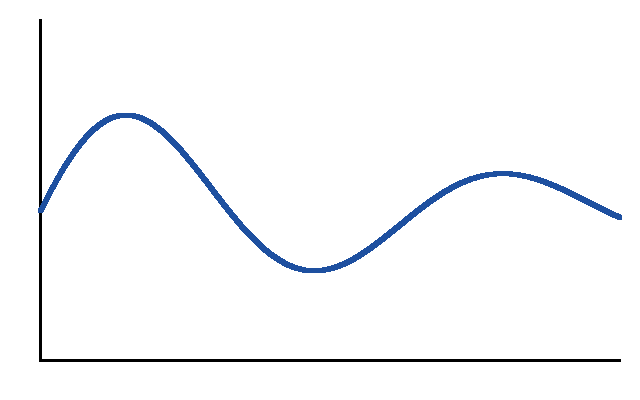
\includegraphics[width=0.7\textwidth]{figures/damped.png}
  \caption{A damped oscillation.}
\end{figure}

\section{Applications of the derivative}

\subsection{Applications of the derivative, part 1}

In this section we study applications of the derivative with care. We begin with the intuition, then state the definitions precisely, and finally prove the main results. Throughout, the reader should keep in mind the geometric picture: a function is a rule, and $f(x)$ describes how that rule behaves as $x \to \infty$. Students often find it useful to work through the examples before reading the proofs, and to return to the proofs once the examples feel familiar. In this section we study applications of the derivative with care. We begin with the intuition, then state the definitions precisely, and finally prove the main results. Throughout, the reader should keep in mind the geometric picture: a function is a rule, and $f(x)$ describes how that rule behaves as $x \to \infty$. Students often find it useful to work through the examples before reading the proofs, and to return to the proofs once the examples feel familiar. 

\begin{equation}
  \lim_{x \to 5} \frac{x^{5} - 5^{5}}{x - 5} = 5 \cdot 5^{4}
  \label{eq:lim3}
\end{equation}

\begin{theorem}
If $f$ is continuous on $[a,b]$ and differentiable on $(a,b)$, then there is a point $c \in (a,b)$ with $f'(c) = \frac{f(b)-f(a)}{b-a}$, as in \eqref{eq:lim3}.
\end{theorem}

\begin{proof}
Apply Rolle's theorem to $g(x) = f(x) - \frac{f(b)-f(a)}{b-a}(x-a)$, which satisfies $g(a) = g(b)$. Then $g'(c) = 0$ for some $c$, and the claim follows.
\end{proof}

In this section we study applications of the derivative with care. We begin with the intuition, then state the definitions precisely, and finally prove the main results. Throughout, the reader should keep in mind the geometric picture: a function is a rule, and $f(x)$ describes how that rule behaves as $x \to \infty$. Students often find it useful to work through the examples before reading the proofs, and to return to the proofs once the examples feel familiar. 

\begin{align}
  \int_0^{5} x^{5}\,dx &= \left[ \frac{x^{6}}{6} \right]_0^{5} \\
  &= \frac{5^{6}}{6} \label{eq:int3}
\end{align}

\begin{itemize}
  \item Compute the limit for $k = 3$.
  \item Check the answer numerically.
  \item Explain why the result is plausible.
\end{itemize}

\subsection{Applications of the derivative, part 2}

In this section we study applications of the derivative with care. We begin with the intuition, then state the definitions precisely, and finally prove the main results. Throughout, the reader should keep in mind the geometric picture: a function is a rule, and $f(x)$ describes how that rule behaves as $x \to \infty$. Students often find it useful to work through the examples before reading the proofs, and to return to the proofs once the examples feel familiar. In this section we study applications of the derivative with care. We begin with the intuition, then state the definitions precisely, and finally prove the main results. Throughout, the reader should keep in mind the geometric picture: a function is a rule, and $f(x)$ describes how that rule behaves as $x \to \infty$. Students often find it useful to work through the examples before reading the proofs, and to return to the proofs once the examples feel familiar. 

\begin{align}
  \int_0^{5} x^{5}\,dx &= \left[ \frac{x^{6}}{6} \right]_0^{5} \\
  &= \frac{5^{6}}{6} \label{eq:int3}
\end{align}

\begin{theorem}
If $f$ is continuous on $[a,b]$ and differentiable on $(a,b)$, then there is a point $c \in (a,b)$ with $f'(c) = \frac{f(b)-f(a)}{b-a}$, as in \eqref{eq:lim3}.
\end{theorem}

\begin{proof}
Apply Rolle's theorem to $g(x) = f(x) - \frac{f(b)-f(a)}{b-a}(x-a)$, which satisfies $g(a) = g(b)$. Then $g'(c) = 0$ for some $c$, and the claim follows.
\end{proof}

In this section we study applications of the derivative with care. We begin with the intuition, then state the definitions precisely, and finally prove the main results. Throughout, the reader should keep in mind the geometric picture: a function is a rule, and $f(x)$ describes how that rule behaves as $x \to \infty$. Students often find it useful to work through the examples before reading the proofs, and to return to the proofs once the examples feel familiar. 

\[
  \sum_{n=1}^{\infty} \frac{1}{n^{5}} \le 1 + \int_1^{\infty} \frac{dx}{x^{5}} = 1 + \frac{1}{4}
\]

\begin{itemize}
  \item Compute the limit for $k = 4$.
  \item Check the answer numerically.
  \item Explain why the result is plausible.
\end{itemize}

\subsection{Applications of the derivative, part 3}

In this section we study applications of the derivative with care. We begin with the intuition, then state the definitions precisely, and finally prove the main results. Throughout, the reader should keep in mind the geometric picture: a function is a rule, and $f(x)$ describes how that rule behaves as $x \to \infty$. Students often find it useful to work through the examples before reading the proofs, and to return to the proofs once the examples feel familiar. In this section we study applications of the derivative with care. We begin with the intuition, then state the definitions precisely, and finally prove the main results. Throughout, the reader should keep in mind the geometric picture: a function is a rule, and $f(x)$ describes how that rule behaves as $x \to \infty$. Students often find it useful to work through the examples before reading the proofs, and to return to the proofs once the examples feel familiar. 

\[
  \sum_{n=1}^{\infty} \frac{1}{n^{5}} \le 1 + \int_1^{\infty} \frac{dx}{x^{5}} = 1 + \frac{1}{4}
\]

\begin{theorem}
If $f$ is continuous on $[a,b]$ and differentiable on $(a,b)$, then there is a point $c \in (a,b)$ with $f'(c) = \frac{f(b)-f(a)}{b-a}$, as in \eqref{eq:lim3}.
\end{theorem}

\begin{proof}
Apply Rolle's theorem to $g(x) = f(x) - \frac{f(b)-f(a)}{b-a}(x-a)$, which satisfies $g(a) = g(b)$. Then $g'(c) = 0$ for some $c$, and the claim follows.
\end{proof}

In this section we study applications of the derivative with care. We begin with the intuition, then state the definitions precisely, and finally prove the main results. Throughout, the reader should keep in mind the geometric picture: a function is a rule, and $f(x)$ describes how that rule behaves as $x \to \infty$. Students often find it useful to work through the examples before reading the proofs, and to return to the proofs once the examples feel familiar. 

\begin{align*}
  (f \circ g)'(x) &= f'(g(x))\, g'(x), \\
  \frac{d}{dx} \sin(5 x) &= 5 \cos(5 x), \\
  \frac{d}{dx} e^{5 x} &= 5 e^{5 x}.
\end{align*}

\begin{itemize}
  \item Compute the limit for $k = 5$.
  \item Check the answer numerically.
  \item Explain why the result is plausible.
\end{itemize}

\section{The definite integral}

\subsection{The definite integral, part 1}

In this section we study the definite integral with care. We begin with the intuition, then state the definitions precisely, and finally prove the main results. Throughout, the reader should keep in mind the geometric picture: a function is a rule, and $\int_a^b f$ describes how that rule behaves as $n \to \infty$. Students often find it useful to work through the examples before reading the proofs, and to return to the proofs once the examples feel familiar. In this section we study the definite integral with care. We begin with the intuition, then state the definitions precisely, and finally prove the main results. Throughout, the reader should keep in mind the geometric picture: a function is a rule, and $\int_a^b f$ describes how that rule behaves as $n \to \infty$. Students often find it useful to work through the examples before reading the proofs, and to return to the proofs once the examples feel familiar. 

\begin{equation}
  \lim_{x \to 6} \frac{x^{6} - 6^{6}}{x - 6} = 6 \cdot 6^{5}
  \label{eq:lim4}
\end{equation}

\begin{theorem}
If $f$ is continuous on $[a,b]$ and differentiable on $(a,b)$, then there is a point $c \in (a,b)$ with $f'(c) = \frac{f(b)-f(a)}{b-a}$, as in \eqref{eq:lim4}.
\end{theorem}

\begin{proof}
Apply Rolle's theorem to $g(x) = f(x) - \frac{f(b)-f(a)}{b-a}(x-a)$, which satisfies $g(a) = g(b)$. Then $g'(c) = 0$ for some $c$, and the claim follows.
\end{proof}

In this section we study the definite integral with care. We begin with the intuition, then state the definitions precisely, and finally prove the main results. Throughout, the reader should keep in mind the geometric picture: a function is a rule, and $\int_a^b f$ describes how that rule behaves as $n \to \infty$. Students often find it useful to work through the examples before reading the proofs, and to return to the proofs once the examples feel familiar. 

\begin{align}
  \int_0^{6} x^{6}\,dx &= \left[ \frac{x^{7}}{7} \right]_0^{6} \\
  &= \frac{6^{7}}{7} \label{eq:int4}
\end{align}

\begin{itemize}
  \item Compute the limit for $k = 4$.
  \item Check the answer numerically.
  \item Explain why the result is plausible.
\end{itemize}

\subsection{The definite integral, part 2}

In this section we study the definite integral with care. We begin with the intuition, then state the definitions precisely, and finally prove the main results. Throughout, the reader should keep in mind the geometric picture: a function is a rule, and $\int_a^b f$ describes how that rule behaves as $n \to \infty$. Students often find it useful to work through the examples before reading the proofs, and to return to the proofs once the examples feel familiar. In this section we study the definite integral with care. We begin with the intuition, then state the definitions precisely, and finally prove the main results. Throughout, the reader should keep in mind the geometric picture: a function is a rule, and $\int_a^b f$ describes how that rule behaves as $n \to \infty$. Students often find it useful to work through the examples before reading the proofs, and to return to the proofs once the examples feel familiar. 

\begin{align}
  \int_0^{6} x^{6}\,dx &= \left[ \frac{x^{7}}{7} \right]_0^{6} \\
  &= \frac{6^{7}}{7} \label{eq:int4}
\end{align}

\begin{theorem}
If $f$ is continuous on $[a,b]$ and differentiable on $(a,b)$, then there is a point $c \in (a,b)$ with $f'(c) = \frac{f(b)-f(a)}{b-a}$, as in \eqref{eq:lim4}.
\end{theorem}

\begin{proof}
Apply Rolle's theorem to $g(x) = f(x) - \frac{f(b)-f(a)}{b-a}(x-a)$, which satisfies $g(a) = g(b)$. Then $g'(c) = 0$ for some $c$, and the claim follows.
\end{proof}

In this section we study the definite integral with care. We begin with the intuition, then state the definitions precisely, and finally prove the main results. Throughout, the reader should keep in mind the geometric picture: a function is a rule, and $\int_a^b f$ describes how that rule behaves as $n \to \infty$. Students often find it useful to work through the examples before reading the proofs, and to return to the proofs once the examples feel familiar. 

\[
  \sum_{n=1}^{\infty} \frac{1}{n^{6}} \le 1 + \int_1^{\infty} \frac{dx}{x^{6}} = 1 + \frac{1}{5}
\]

\begin{itemize}
  \item Compute the limit for $k = 5$.
  \item Check the answer numerically.
  \item Explain why the result is plausible.
\end{itemize}

\subsection{The definite integral, part 3}

In this section we study the definite integral with care. We begin with the intuition, then state the definitions precisely, and finally prove the main results. Throughout, the reader should keep in mind the geometric picture: a function is a rule, and $\int_a^b f$ describes how that rule behaves as $n \to \infty$. Students often find it useful to work through the examples before reading the proofs, and to return to the proofs once the examples feel familiar. In this section we study the definite integral with care. We begin with the intuition, then state the definitions precisely, and finally prove the main results. Throughout, the reader should keep in mind the geometric picture: a function is a rule, and $\int_a^b f$ describes how that rule behaves as $n \to \infty$. Students often find it useful to work through the examples before reading the proofs, and to return to the proofs once the examples feel familiar. 

\[
  \sum_{n=1}^{\infty} \frac{1}{n^{6}} \le 1 + \int_1^{\infty} \frac{dx}{x^{6}} = 1 + \frac{1}{5}
\]

\begin{theorem}
If $f$ is continuous on $[a,b]$ and differentiable on $(a,b)$, then there is a point $c \in (a,b)$ with $f'(c) = \frac{f(b)-f(a)}{b-a}$, as in \eqref{eq:lim4}.
\end{theorem}

\begin{proof}
Apply Rolle's theorem to $g(x) = f(x) - \frac{f(b)-f(a)}{b-a}(x-a)$, which satisfies $g(a) = g(b)$. Then $g'(c) = 0$ for some $c$, and the claim follows.
\end{proof}

In this section we study the definite integral with care. We begin with the intuition, then state the definitions precisely, and finally prove the main results. Throughout, the reader should keep in mind the geometric picture: a function is a rule, and $\int_a^b f$ describes how that rule behaves as $n \to \infty$. Students often find it useful to work through the examples before reading the proofs, and to return to the proofs once the examples feel familiar. 

\begin{align*}
  (f \circ g)'(x) &= f'(g(x))\, g'(x), \\
  \frac{d}{dx} \sin(6 x) &= 6 \cos(6 x), \\
  \frac{d}{dx} e^{6 x} &= 6 e^{6 x}.
\end{align*}

\begin{itemize}
  \item Compute the limit for $k = 6$.
  \item Check the answer numerically.
  \item Explain why the result is plausible.
\end{itemize}

\begin{figure}[ht]
  \centering
  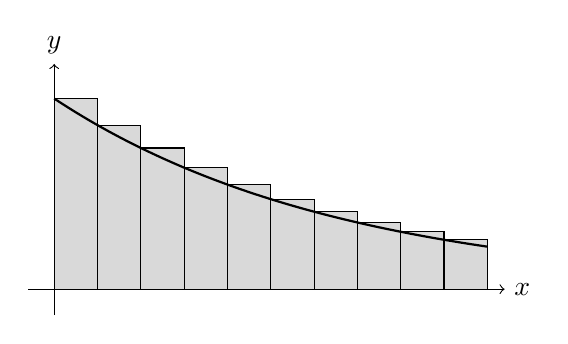
\begin{tikzpicture}[scale=1.1]
    \draw[->] (-0.3,0) -- (5.2,0) node[right] {$x$};
    \draw[->] (0,-0.3) -- (0,2.6) node[above] {$y$};
    \foreach \i in {0,...,9} {
      \pgfmathsetmacro{\x}{0.5*\i}
      \pgfmathsetmacro{\h}{2.2*exp(-0.3*\x)}
      \draw[fill=gray!30] (\x,0) rectangle ++(0.5,\h);
    }
    \draw[thick,domain=0:5,smooth,variable=\x] plot ({\x},{2.2*exp(-0.3*\x)});
  \end{tikzpicture}
  \caption{A Riemann sum with ten rectangles.}
\end{figure}

\section{Techniques of integration}

\subsection{Techniques of integration, part 1}

In this section we study techniques of integration with care. We begin with the intuition, then state the definitions precisely, and finally prove the main results. Throughout, the reader should keep in mind the geometric picture: a function is a rule, and $\int u\,dv$ describes how that rule behaves as $x \to 1$. Students often find it useful to work through the examples before reading the proofs, and to return to the proofs once the examples feel familiar. In this section we study techniques of integration with care. We begin with the intuition, then state the definitions precisely, and finally prove the main results. Throughout, the reader should keep in mind the geometric picture: a function is a rule, and $\int u\,dv$ describes how that rule behaves as $x \to 1$. Students often find it useful to work through the examples before reading the proofs, and to return to the proofs once the examples feel familiar. 

\begin{equation}
  \lim_{x \to 7} \frac{x^{7} - 7^{7}}{x - 7} = 7 \cdot 7^{6}
  \label{eq:lim5}
\end{equation}

\begin{theorem}
If $f$ is continuous on $[a,b]$ and differentiable on $(a,b)$, then there is a point $c \in (a,b)$ with $f'(c) = \frac{f(b)-f(a)}{b-a}$, as in \eqref{eq:lim5}.
\end{theorem}

\begin{proof}
Apply Rolle's theorem to $g(x) = f(x) - \frac{f(b)-f(a)}{b-a}(x-a)$, which satisfies $g(a) = g(b)$. Then $g'(c) = 0$ for some $c$, and the claim follows.
\end{proof}

In this section we study techniques of integration with care. We begin with the intuition, then state the definitions precisely, and finally prove the main results. Throughout, the reader should keep in mind the geometric picture: a function is a rule, and $\int u\,dv$ describes how that rule behaves as $x \to 1$. Students often find it useful to work through the examples before reading the proofs, and to return to the proofs once the examples feel familiar. 

\begin{align}
  \int_0^{7} x^{7}\,dx &= \left[ \frac{x^{8}}{8} \right]_0^{7} \\
  &= \frac{7^{8}}{8} \label{eq:int5}
\end{align}

\begin{itemize}
  \item Compute the limit for $k = 5$.
  \item Check the answer numerically.
  \item Explain why the result is plausible.
\end{itemize}

\subsection{Techniques of integration, part 2}

In this section we study techniques of integration with care. We begin with the intuition, then state the definitions precisely, and finally prove the main results. Throughout, the reader should keep in mind the geometric picture: a function is a rule, and $\int u\,dv$ describes how that rule behaves as $x \to 1$. Students often find it useful to work through the examples before reading the proofs, and to return to the proofs once the examples feel familiar. In this section we study techniques of integration with care. We begin with the intuition, then state the definitions precisely, and finally prove the main results. Throughout, the reader should keep in mind the geometric picture: a function is a rule, and $\int u\,dv$ describes how that rule behaves as $x \to 1$. Students often find it useful to work through the examples before reading the proofs, and to return to the proofs once the examples feel familiar. 

\begin{align}
  \int_0^{7} x^{7}\,dx &= \left[ \frac{x^{8}}{8} \right]_0^{7} \\
  &= \frac{7^{8}}{8} \label{eq:int5}
\end{align}

\begin{theorem}
If $f$ is continuous on $[a,b]$ and differentiable on $(a,b)$, then there is a point $c \in (a,b)$ with $f'(c) = \frac{f(b)-f(a)}{b-a}$, as in \eqref{eq:lim5}.
\end{theorem}

\begin{proof}
Apply Rolle's theorem to $g(x) = f(x) - \frac{f(b)-f(a)}{b-a}(x-a)$, which satisfies $g(a) = g(b)$. Then $g'(c) = 0$ for some $c$, and the claim follows.
\end{proof}

In this section we study techniques of integration with care. We begin with the intuition, then state the definitions precisely, and finally prove the main results. Throughout, the reader should keep in mind the geometric picture: a function is a rule, and $\int u\,dv$ describes how that rule behaves as $x \to 1$. Students often find it useful to work through the examples before reading the proofs, and to return to the proofs once the examples feel familiar. 

\[
  \sum_{n=1}^{\infty} \frac{1}{n^{7}} \le 1 + \int_1^{\infty} \frac{dx}{x^{7}} = 1 + \frac{1}{6}
\]

\begin{itemize}
  \item Compute the limit for $k = 6$.
  \item Check the answer numerically.
  \item Explain why the result is plausible.
\end{itemize}

\subsection{Techniques of integration, part 3}

In this section we study techniques of integration with care. We begin with the intuition, then state the definitions precisely, and finally prove the main results. Throughout, the reader should keep in mind the geometric picture: a function is a rule, and $\int u\,dv$ describes how that rule behaves as $x \to 1$. Students often find it useful to work through the examples before reading the proofs, and to return to the proofs once the examples feel familiar. In this section we study techniques of integration with care. We begin with the intuition, then state the definitions precisely, and finally prove the main results. Throughout, the reader should keep in mind the geometric picture: a function is a rule, and $\int u\,dv$ describes how that rule behaves as $x \to 1$. Students often find it useful to work through the examples before reading the proofs, and to return to the proofs once the examples feel familiar. 

\[
  \sum_{n=1}^{\infty} \frac{1}{n^{7}} \le 1 + \int_1^{\infty} \frac{dx}{x^{7}} = 1 + \frac{1}{6}
\]

\begin{theorem}
If $f$ is continuous on $[a,b]$ and differentiable on $(a,b)$, then there is a point $c \in (a,b)$ with $f'(c) = \frac{f(b)-f(a)}{b-a}$, as in \eqref{eq:lim5}.
\end{theorem}

\begin{proof}
Apply Rolle's theorem to $g(x) = f(x) - \frac{f(b)-f(a)}{b-a}(x-a)$, which satisfies $g(a) = g(b)$. Then $g'(c) = 0$ for some $c$, and the claim follows.
\end{proof}

In this section we study techniques of integration with care. We begin with the intuition, then state the definitions precisely, and finally prove the main results. Throughout, the reader should keep in mind the geometric picture: a function is a rule, and $\int u\,dv$ describes how that rule behaves as $x \to 1$. Students often find it useful to work through the examples before reading the proofs, and to return to the proofs once the examples feel familiar. 

\begin{align*}
  (f \circ g)'(x) &= f'(g(x))\, g'(x), \\
  \frac{d}{dx} \sin(7 x) &= 7 \cos(7 x), \\
  \frac{d}{dx} e^{7 x} &= 7 e^{7 x}.
\end{align*}

\begin{itemize}
  \item Compute the limit for $k = 7$.
  \item Check the answer numerically.
  \item Explain why the result is plausible.
\end{itemize}

\section{Sequences and series}

\subsection{Sequences and series, part 1}

In this section we study sequences and series with care. We begin with the intuition, then state the definitions precisely, and finally prove the main results. Throughout, the reader should keep in mind the geometric picture: a function is a rule, and $a_n$ describes how that rule behaves as $n \to \infty$. Students often find it useful to work through the examples before reading the proofs, and to return to the proofs once the examples feel familiar. In this section we study sequences and series with care. We begin with the intuition, then state the definitions precisely, and finally prove the main results. Throughout, the reader should keep in mind the geometric picture: a function is a rule, and $a_n$ describes how that rule behaves as $n \to \infty$. Students often find it useful to work through the examples before reading the proofs, and to return to the proofs once the examples feel familiar. 

\begin{equation}
  \lim_{x \to 8} \frac{x^{8} - 8^{8}}{x - 8} = 8 \cdot 8^{7}
  \label{eq:lim6}
\end{equation}

\begin{theorem}
If $f$ is continuous on $[a,b]$ and differentiable on $(a,b)$, then there is a point $c \in (a,b)$ with $f'(c) = \frac{f(b)-f(a)}{b-a}$, as in \eqref{eq:lim6}.
\end{theorem}

\begin{proof}
Apply Rolle's theorem to $g(x) = f(x) - \frac{f(b)-f(a)}{b-a}(x-a)$, which satisfies $g(a) = g(b)$. Then $g'(c) = 0$ for some $c$, and the claim follows.
\end{proof}

In this section we study sequences and series with care. We begin with the intuition, then state the definitions precisely, and finally prove the main results. Throughout, the reader should keep in mind the geometric picture: a function is a rule, and $a_n$ describes how that rule behaves as $n \to \infty$. Students often find it useful to work through the examples before reading the proofs, and to return to the proofs once the examples feel familiar. 

\begin{align}
  \int_0^{8} x^{8}\,dx &= \left[ \frac{x^{9}}{9} \right]_0^{8} \\
  &= \frac{8^{9}}{9} \label{eq:int6}
\end{align}

\begin{itemize}
  \item Compute the limit for $k = 6$.
  \item Check the answer numerically.
  \item Explain why the result is plausible.
\end{itemize}

\subsection{Sequences and series, part 2}

In this section we study sequences and series with care. We begin with the intuition, then state the definitions precisely, and finally prove the main results. Throughout, the reader should keep in mind the geometric picture: a function is a rule, and $a_n$ describes how that rule behaves as $n \to \infty$. Students often find it useful to work through the examples before reading the proofs, and to return to the proofs once the examples feel familiar. In this section we study sequences and series with care. We begin with the intuition, then state the definitions precisely, and finally prove the main results. Throughout, the reader should keep in mind the geometric picture: a function is a rule, and $a_n$ describes how that rule behaves as $n \to \infty$. Students often find it useful to work through the examples before reading the proofs, and to return to the proofs once the examples feel familiar. 

\begin{align}
  \int_0^{8} x^{8}\,dx &= \left[ \frac{x^{9}}{9} \right]_0^{8} \\
  &= \frac{8^{9}}{9} \label{eq:int6}
\end{align}

\begin{theorem}
If $f$ is continuous on $[a,b]$ and differentiable on $(a,b)$, then there is a point $c \in (a,b)$ with $f'(c) = \frac{f(b)-f(a)}{b-a}$, as in \eqref{eq:lim6}.
\end{theorem}

\begin{proof}
Apply Rolle's theorem to $g(x) = f(x) - \frac{f(b)-f(a)}{b-a}(x-a)$, which satisfies $g(a) = g(b)$. Then $g'(c) = 0$ for some $c$, and the claim follows.
\end{proof}

In this section we study sequences and series with care. We begin with the intuition, then state the definitions precisely, and finally prove the main results. Throughout, the reader should keep in mind the geometric picture: a function is a rule, and $a_n$ describes how that rule behaves as $n \to \infty$. Students often find it useful to work through the examples before reading the proofs, and to return to the proofs once the examples feel familiar. 

\[
  \sum_{n=1}^{\infty} \frac{1}{n^{8}} \le 1 + \int_1^{\infty} \frac{dx}{x^{8}} = 1 + \frac{1}{7}
\]

\begin{itemize}
  \item Compute the limit for $k = 7$.
  \item Check the answer numerically.
  \item Explain why the result is plausible.
\end{itemize}

\subsection{Sequences and series, part 3}

In this section we study sequences and series with care. We begin with the intuition, then state the definitions precisely, and finally prove the main results. Throughout, the reader should keep in mind the geometric picture: a function is a rule, and $a_n$ describes how that rule behaves as $n \to \infty$. Students often find it useful to work through the examples before reading the proofs, and to return to the proofs once the examples feel familiar. In this section we study sequences and series with care. We begin with the intuition, then state the definitions precisely, and finally prove the main results. Throughout, the reader should keep in mind the geometric picture: a function is a rule, and $a_n$ describes how that rule behaves as $n \to \infty$. Students often find it useful to work through the examples before reading the proofs, and to return to the proofs once the examples feel familiar. 

\[
  \sum_{n=1}^{\infty} \frac{1}{n^{8}} \le 1 + \int_1^{\infty} \frac{dx}{x^{8}} = 1 + \frac{1}{7}
\]

\begin{theorem}
If $f$ is continuous on $[a,b]$ and differentiable on $(a,b)$, then there is a point $c \in (a,b)$ with $f'(c) = \frac{f(b)-f(a)}{b-a}$, as in \eqref{eq:lim6}.
\end{theorem}

\begin{proof}
Apply Rolle's theorem to $g(x) = f(x) - \frac{f(b)-f(a)}{b-a}(x-a)$, which satisfies $g(a) = g(b)$. Then $g'(c) = 0$ for some $c$, and the claim follows.
\end{proof}

In this section we study sequences and series with care. We begin with the intuition, then state the definitions precisely, and finally prove the main results. Throughout, the reader should keep in mind the geometric picture: a function is a rule, and $a_n$ describes how that rule behaves as $n \to \infty$. Students often find it useful to work through the examples before reading the proofs, and to return to the proofs once the examples feel familiar. 

\begin{align*}
  (f \circ g)'(x) &= f'(g(x))\, g'(x), \\
  \frac{d}{dx} \sin(8 x) &= 8 \cos(8 x), \\
  \frac{d}{dx} e^{8 x} &= 8 e^{8 x}.
\end{align*}

\begin{itemize}
  \item Compute the limit for $k = 8$.
  \item Check the answer numerically.
  \item Explain why the result is plausible.
\end{itemize}

\begin{figure}[ht]
  \centering
  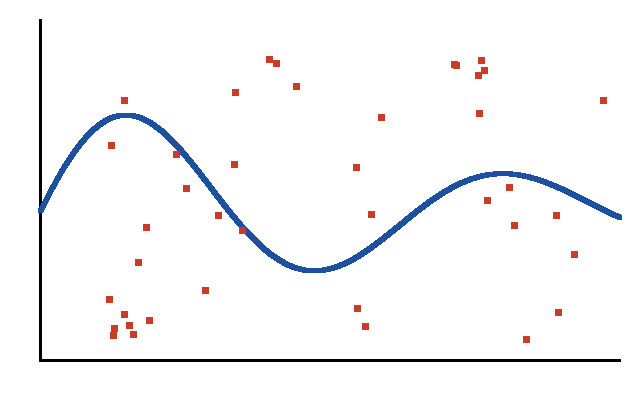
\includegraphics[width=0.7\textwidth]{figures/scatter.jpg}
  \caption{Measured values around a curve.}
\end{figure}

\section{Power series}

\subsection{Power series, part 1}

In this section we study power series with care. We begin with the intuition, then state the definitions precisely, and finally prove the main results. Throughout, the reader should keep in mind the geometric picture: a function is a rule, and $\sum c_n x^n$ describes how that rule behaves as $|x| \to R$. Students often find it useful to work through the examples before reading the proofs, and to return to the proofs once the examples feel familiar. In this section we study power series with care. We begin with the intuition, then state the definitions precisely, and finally prove the main results. Throughout, the reader should keep in mind the geometric picture: a function is a rule, and $\sum c_n x^n$ describes how that rule behaves as $|x| \to R$. Students often find it useful to work through the examples before reading the proofs, and to return to the proofs once the examples feel familiar. 

\begin{equation}
  \lim_{x \to 9} \frac{x^{9} - 9^{9}}{x - 9} = 9 \cdot 9^{8}
  \label{eq:lim7}
\end{equation}

\begin{theorem}
If $f$ is continuous on $[a,b]$ and differentiable on $(a,b)$, then there is a point $c \in (a,b)$ with $f'(c) = \frac{f(b)-f(a)}{b-a}$, as in \eqref{eq:lim7}.
\end{theorem}

\begin{proof}
Apply Rolle's theorem to $g(x) = f(x) - \frac{f(b)-f(a)}{b-a}(x-a)$, which satisfies $g(a) = g(b)$. Then $g'(c) = 0$ for some $c$, and the claim follows.
\end{proof}

In this section we study power series with care. We begin with the intuition, then state the definitions precisely, and finally prove the main results. Throughout, the reader should keep in mind the geometric picture: a function is a rule, and $\sum c_n x^n$ describes how that rule behaves as $|x| \to R$. Students often find it useful to work through the examples before reading the proofs, and to return to the proofs once the examples feel familiar. 

\begin{align}
  \int_0^{9} x^{9}\,dx &= \left[ \frac{x^{10}}{10} \right]_0^{9} \\
  &= \frac{9^{10}}{10} \label{eq:int7}
\end{align}

\begin{itemize}
  \item Compute the limit for $k = 7$.
  \item Check the answer numerically.
  \item Explain why the result is plausible.
\end{itemize}

\subsection{Power series, part 2}

In this section we study power series with care. We begin with the intuition, then state the definitions precisely, and finally prove the main results. Throughout, the reader should keep in mind the geometric picture: a function is a rule, and $\sum c_n x^n$ describes how that rule behaves as $|x| \to R$. Students often find it useful to work through the examples before reading the proofs, and to return to the proofs once the examples feel familiar. In this section we study power series with care. We begin with the intuition, then state the definitions precisely, and finally prove the main results. Throughout, the reader should keep in mind the geometric picture: a function is a rule, and $\sum c_n x^n$ describes how that rule behaves as $|x| \to R$. Students often find it useful to work through the examples before reading the proofs, and to return to the proofs once the examples feel familiar. 

\begin{align}
  \int_0^{9} x^{9}\,dx &= \left[ \frac{x^{10}}{10} \right]_0^{9} \\
  &= \frac{9^{10}}{10} \label{eq:int7}
\end{align}

\begin{theorem}
If $f$ is continuous on $[a,b]$ and differentiable on $(a,b)$, then there is a point $c \in (a,b)$ with $f'(c) = \frac{f(b)-f(a)}{b-a}$, as in \eqref{eq:lim7}.
\end{theorem}

\begin{proof}
Apply Rolle's theorem to $g(x) = f(x) - \frac{f(b)-f(a)}{b-a}(x-a)$, which satisfies $g(a) = g(b)$. Then $g'(c) = 0$ for some $c$, and the claim follows.
\end{proof}

In this section we study power series with care. We begin with the intuition, then state the definitions precisely, and finally prove the main results. Throughout, the reader should keep in mind the geometric picture: a function is a rule, and $\sum c_n x^n$ describes how that rule behaves as $|x| \to R$. Students often find it useful to work through the examples before reading the proofs, and to return to the proofs once the examples feel familiar. 

\[
  \sum_{n=1}^{\infty} \frac{1}{n^{9}} \le 1 + \int_1^{\infty} \frac{dx}{x^{9}} = 1 + \frac{1}{8}
\]

\begin{itemize}
  \item Compute the limit for $k = 8$.
  \item Check the answer numerically.
  \item Explain why the result is plausible.
\end{itemize}

\subsection{Power series, part 3}

In this section we study power series with care. We begin with the intuition, then state the definitions precisely, and finally prove the main results. Throughout, the reader should keep in mind the geometric picture: a function is a rule, and $\sum c_n x^n$ describes how that rule behaves as $|x| \to R$. Students often find it useful to work through the examples before reading the proofs, and to return to the proofs once the examples feel familiar. In this section we study power series with care. We begin with the intuition, then state the definitions precisely, and finally prove the main results. Throughout, the reader should keep in mind the geometric picture: a function is a rule, and $\sum c_n x^n$ describes how that rule behaves as $|x| \to R$. Students often find it useful to work through the examples before reading the proofs, and to return to the proofs once the examples feel familiar. 

\[
  \sum_{n=1}^{\infty} \frac{1}{n^{9}} \le 1 + \int_1^{\infty} \frac{dx}{x^{9}} = 1 + \frac{1}{8}
\]

\begin{theorem}
If $f$ is continuous on $[a,b]$ and differentiable on $(a,b)$, then there is a point $c \in (a,b)$ with $f'(c) = \frac{f(b)-f(a)}{b-a}$, as in \eqref{eq:lim7}.
\end{theorem}

\begin{proof}
Apply Rolle's theorem to $g(x) = f(x) - \frac{f(b)-f(a)}{b-a}(x-a)$, which satisfies $g(a) = g(b)$. Then $g'(c) = 0$ for some $c$, and the claim follows.
\end{proof}

In this section we study power series with care. We begin with the intuition, then state the definitions precisely, and finally prove the main results. Throughout, the reader should keep in mind the geometric picture: a function is a rule, and $\sum c_n x^n$ describes how that rule behaves as $|x| \to R$. Students often find it useful to work through the examples before reading the proofs, and to return to the proofs once the examples feel familiar. 

\begin{align*}
  (f \circ g)'(x) &= f'(g(x))\, g'(x), \\
  \frac{d}{dx} \sin(9 x) &= 9 \cos(9 x), \\
  \frac{d}{dx} e^{9 x} &= 9 e^{9 x}.
\end{align*}

\begin{itemize}
  \item Compute the limit for $k = 9$.
  \item Check the answer numerically.
  \item Explain why the result is plausible.
\end{itemize}

\end{document}
